%% paper.tex -- Astronomy & Astrophysics (A&A) manuscript
%%
%% Uses the official A&A LaTeX class and bibliography style (aa.cls,
%% aa.bst, plus the lineno/linenoaa support files), included in this
%% repository alongside this file. Compiles with:
%%   pdflatex paper && bibtex paper && pdflatex paper && pdflatex paper
%%
\documentclass{aa}

% txfonts gives the Times-based text/math faces standard in published A&A
% articles (the default Computer/Latin Modern faces read as generic LaTeX
% output). It also supplies full scalable T1 outlines itself, so it
% incidentally avoids the low-resolution bitmap-font fallback aa.cls's
% forced T1 encoding can otherwise trigger.
\usepackage{txfonts}
\usepackage{graphicx}
\usepackage{amsmath}
\usepackage{amssymb}

\begin{document}

\title{Impact of Solar Orbiter polar-view magnetic constraints on surface flux transport estimates of the Sun's axial dipole moment}

\author{M.~H.~Talafha\inst{1,2}}

\institute{
Research Institute of Sciences and Engineering, University of Sharjah, Sharjah, United Arab Emirates\\
\email{mtalafha901@gmail.com}
\and
HUN-REN Wigner Research Centre for Physics, Budapest, Hungary
}

% Fill in once known from the editorial office.
\date{Received ---; accepted ---}

\abstract
{The Sun's axial dipole moment $g_{10}$ is the strongest observational precursor of the next solar cycle's amplitude, and the quantity a surface flux transport (SFT) model must be initialised with. Its value is set by the polar field, precisely the region near-ecliptic magnetographs such as SDO/HMI never observe at favourable angles.}
{We ask whether the out-of-ecliptic vantage of Solar Orbiter/PHI measurably improves polar-field coverage and the resulting SFT prediction, relative to Earth-view data alone.}
{Using a common, open-source pipeline that builds PHI-only, HMI-only (native Earth-view geometry), and merged Carrington maps and computes $g_{10}$ under three polar-filling assumptions, we analyse a low-inclination demonstration window (Carrington rotation, CR, 2264, 2022) and the decisive high-$B_0$ campaign of February--July 2025 (CR\,2294--2299), during which Solar Orbiter's disk-centre latitude $B_0$ swept from $-2^{\circ}$ through $-16.7^{\circ}$ to $+16.8^{\circ}$ and back.}
{PHI's $\ge 60^{\circ}$ polar-cap coverage overtakes HMI by up to a factor of 16 (north cap 51\% versus 3\% in April 2025); the advantage switches on and off with $|B_0|$ exactly as predicted and, crucially, is largest precisely when the Solar Orbiter--Earth longitude separation is largest, so a per-pixel map merge is invalid at the decisive epochs. Injecting PHI's north-cap field into the SFT initial condition where HMI is effectively blind shifts the first predicted polar reversal by $-1.68$\,yr; injecting its co-observed south-cap field, where HMI already sees the pole, changes the timing by only $-0.004$\,yr.}
{The polar view alters the flux-transport prediction only where the Earth view lacks the information: Solar Orbiter/PHI's value lies not as a co-registered merge partner for HMI, but as a standalone polar boundary constraint when Earth-based magnetographs cannot see a given pole. The two vantages are complementary in time, not in space.}

\keywords{Sun: magnetic fields -- Sun: photosphere -- Sun: activity -- Sun: heliosphere -- methods: data analysis -- instrumentation: polarimeters}

\titlerunning{Solar Orbiter/PHI polar constraints on the axial dipole}
\authorrunning{M.~H.~Talafha}

\maketitle

%-------------------------------------------------------------------
\section{Introduction}
\label{sec:introduction}

The polar magnetic field near solar minimum is the best-known precursor of the amplitude of the next sunspot cycle \citep{Svalgaard2005,Petrovay2020}, and its low-order proxy -- the axial dipole moment
\begin{equation}
    g_{10} = \frac{3}{4\pi} \oint B_r \sin\lambda \, \mathrm{d}\Omega
    \label{eq:g10-intro}
\end{equation}
-- is the natural summary quantity, because it is what surface flux transport (SFT) models propagate forward \citep{Babcock1961,Leighton1969,Sheeley2005,WangSheeley1991,Wang2017}. Any error in the polar field therefore propagates directly into cycle-amplitude forecasts, since the surface polar field is itself the source from which the dynamo builds the next cycle's toroidal field \citep{CameronSchussler2015}.

The polar field is also the hardest part of the Sun to measure. From the ecliptic the poles are seen at grazing angle ($\mu = \cos\theta \to 0$, where $\theta$ is the heliocentric angle), so the line-of-sight field there is a large and uncertain extrapolation, and for months around each equinox a pole is tilted away from Earth entirely. Standard synoptic products (e.g.\ \texttt{hmi.synoptic\_mr\_polfil\_720s}) fill the polar caps with a temporal/spatial model rather than a contemporaneous measurement \citep{Sun2018}. The polar contribution to $g_{10}$ is thus, to a significant degree, an assumption rather than an observation.

Solar Orbiter \citep{Muller2020}, whose orbit is progressively inclined out of the ecliptic by successive Venus gravity assists, carries the Polarimetric and Helioseismic Imager (PHI; \citealp{Solanki2020}) and provides the first opportunity to view the solar poles at favourable angles from a second vantage. This paper asks a specific, falsifiable question: \emph{does adding PHI's polar-view magnetic information measurably improve the estimate of $g_{10}$ and the SFT prediction that follows from it, relative to Earth-view data alone?} We answer it with a single open-source pipeline applied to two windows -- a 2022 low-inclination demonstration and the high-inclination campaign of 2025 -- and arrive at a reframing of \emph{how} the two vantages are best combined.

The paper is organised as follows. Section~\ref{sec:data} describes the SO/PHI-FDT and SDO/HMI observations and the two analysis windows. Section~\ref{sec:methods} sets out the map-merging, radial-field, and dipole-estimation methodology, together with the SFT model. Section~\ref{sec:results} presents the results, from the 2022 method demonstration to the decisive 2025 campaign. Sections~\ref{sec:discussion}--\ref{sec:conclusions} discuss the results, list the main uncertainties, and draw conclusions.

%-------------------------------------------------------------------
\section{Observations and data preparation}
\label{sec:data}

We use SO/PHI-FDT line-of-sight (\texttt{blos}) Level-2 magnetograms and matched SDO/HMI \texttt{hmi.M\_720s} magnetograms. For each PHI frame the nearest HMI record in time is selected and rejected if the offset exceeds a threshold of 600\,s.

\subsection{SO/PHI-FDT line-of-sight magnetograms}
\label{sec:data-phi}

The Full Disc Telescope (FDT) channel of the Polarimetric and Helioseismic Imager aboard Solar Orbiter \citep{Solanki2020} provides Level-2 full-disk line-of-sight magnetic field maps, identified by the observable name \texttt{blos}. The line-of-sight field is computed on the ground from the magnetic field magnitude and inclination delivered by the radiative-transfer inversion pipeline; the same data release also provides continuum intensity, full Stokes data, line-of-sight velocity, and the full vector magnetic field, but only \texttt{blos} is used here. SO/PHI data combine on-board pre-processing and inversion with ground-based calibration to physical units and FITS-metadata assembly.

The SO/PHI-FDT observations processed here span two observing programmes and, for a subset of files, ship without the \texttt{CUNIT1}/\texttt{CUNIT2} FITS keywords; these units are patched automatically on load. Datasets acquired from 22~February 2025 onwards are generally on-board averages of three individual measurements taken to improve the signal-to-noise ratio, and residual artefacts (telemetry gaps, focus changes, imperfect flat-fielding, ghost and fringe signatures, a dust-grain imprint most visible in continuum intensity) can remain, which is a relevant caveat for subtle spatial differences between PHI and HMI in the weak-signal regime.

Each PHI magnetogram is treated as the reference observation of a matched PHI--HMI pair, and the nearest HMI magnetogram is later reprojected onto the PHI image grid. This preserves the Solar Orbiter viewing geometry throughout the analysis.

\subsection{SDO/HMI line-of-sight magnetograms}
\label{sec:data-hmi}

For the Earth-view reference we use line-of-sight magnetograms from the Helioseismic and Magnetic Imager \citep[HMI;][]{Scherrer2012} aboard the Solar Dynamics Observatory \citep[SDO;][]{Pesnell2012}, specifically the \texttt{hmi.M\_720s} data series. HMI observes the same Fe\,\textsc{i} 6173\,\AA\ line as SO/PHI, at a cadence suitable for matching to the available PHI-FDT observations.

Unlike the PHI data, the HMI magnetograms used for the merged and reprojected products are not analysed in their native image plane: they are reprojected onto the PHI grid using the World Coordinate System (WCS) information in the FITS headers \citep{Thompson2006} before any blending or dipole estimation. For the native-geometry HMI-only product (Sect.~\ref{sec:methods-merge}), by contrast, HMI is kept in its own disk geometry, so that the vantage comparison with PHI is not made circular by forcing both products through the same grid.

\subsection{The two observing windows}
\label{sec:data-windows}

Two windows are analysed (Table~\ref{tab:obs}). The first is a compact, low-inclination demonstration window covering Carrington Rotation (CR) 2264, 27~October--3~November 2022, with 24 matched PHI--HMI cases drawn from two observing programmes; 18 of the 24 cases have a time offset $|\Delta t| \le 3$\,s, with a maximum of 189\,s. Over this window Solar Orbiter's heliographic latitude of disk centre, $B_0^{\rm SolO}$, ran from $+7.09^{\circ}$ to $+7.44^{\circ}$ against Earth's $B_0^{\oplus} = +4.72^{\circ}$ to $+4.88^{\circ}$, with Solar Orbiter trailing Earth by $40^{\circ}$--$45^{\circ}$ in Carrington longitude -- a small polar-viewing advantage that mainly exercises the pipeline machinery.

The second is the decisive high-$B_0$ campaign of 14~February--16~July 2025, spanning six Carrington rotations, CR\,2294--2299, with essentially simultaneous PHI--HMI matches ($|\Delta t| = 2$--3\,s). Over this interval $B_0^{\rm SolO}$ swept from near-ecliptic ($-2^{\circ}$) to a deep southern view ($-16.7^{\circ}$, late March), up to a northern plateau ($+16.8^{\circ}$, late April--May), and back down towards the ecliptic through June--July, while $B_0^{\oplus}$ rose from $-7^{\circ}$ towards $-2^{\circ}$ (northern summer). The Solar Orbiter--Earth Carrington-longitude separation ranges from $0.3^{\circ}$ (a near-conjunction in mid-March) to $168^{\circ}$--$180^{\circ}$ (the CR\,2297 apex, essentially opposite hemispheres); a single rotation can carry more than 200 matched cases (203 for CR\,2297).

\begin{table}
\caption{Summary of the two observing windows.}
\label{tab:obs}
\centering
\begin{tabular}{lll}
\hline\hline
Property & CR\,2264 (2022) & 2025 campaign \\
\hline
Rotations & CR\,2264 & CR\,2294--2299 \\
Start & 2022-10-27 & 2025-02-14 \\
End & 2022-11-03 & 2025-07-16 \\
Matched cases & 24 & up to 203/rotation \\
Match tolerance & 600\,s & 600\,s \\
Typical $|\Delta t|$ & $\le 3$\,s\tablefootmark{a} & 2--3\,s \\
$B_0^{\rm SolO}$ range & $+7.1^{\circ}$ to $+7.4^{\circ}$ & $-16.7^{\circ}$ to $+16.8^{\circ}$ \\
$B_0^{\oplus}$ range & $+4.7^{\circ}$ to $+4.9^{\circ}$ & $-7^{\circ}$ to $-2^{\circ}$ \\
Separation & $40^{\circ}$--$45^{\circ}$ & $0.3^{\circ}$--$180^{\circ}$ \\
\hline
\end{tabular}
\tablefoot{
\tablefoottext{a}{For 18 of 24 cases; the remaining cases reach a maximum offset of 189\,s.}
}
\end{table}

\subsection{Time matching and viewing-geometry systematics}
\label{sec:data-systematics}

Two viewing-geometry systematics are handled explicitly. First, HMI's camera carries a $\approx 180^{\circ}$ \texttt{CROTA2} rotation; the native-geometry map path honours this through the full PC/CROTA orientation, and ignoring it mirrors the map between hemispheres and flips the sign of $g_{10}$ (a $-2.11 \rightarrow +2.20$\,G swing on the CR\,2264 subset in project mode) -- a cautionary systematic for any direct-geometry synoptic construction. Second, the line-of-sight field is converted to an approximate radial field as $B_r \approx B_{\rm los}/\mu^{\alpha}$ with a limb cut $\mu \ge \mu_{\rm min}$ (Sect.~\ref{sec:methods-radial}).

Per-case cross-calibration (through-origin regression over pixels with $|B|$ above a floor and $\mu \ge \mu_{\rm min}$) is computed for every case as a slope and Pearson correlation coefficient $r$. Over the CR\,2264 window the slope declines monotonically from 0.75 to 0.50 across eight days at a stable $r \approx 0.75$, tracking the Solar Orbiter--Sun distance nearly linearly. In the 2025 campaign the slope is $\approx 0.55$ with $r \approx 0.8$ while the two spacecraft co-observe, and both the correlation and the slope collapse ($r \rightarrow 0.44$, slope $\rightarrow 0.31$) once the Solar Orbiter--Earth separation grows past $\approx 55^{\circ}$, as the co-observed disk shrinks towards the limb. Calibration is applied only when explicitly requested and only when $r$ exceeds a floor (default 0.5), and only when the two spacecraft actually co-observe.

The sub-unity slope is a \emph{resolution} effect, not an instrument-scale or vantage error. Re-running the regression on the 112 co-observing 2025 cases with the HMI map progressively smoothed, the mean slope climbs monotonically from 0.56 to 0.63, 0.80, 0.88, 0.98, and 1.08 at Gaussian FWHM 0, 1, 2, 3, 5, and 8 PHI-grid pixels, respectively, crossing unity near 5\,px, while the correlation peaks ($r \approx 0.93$) at FWHM 2--3\,px. This is the signature of PHI's coarser plate scale: fine mixed-polarity structure cancels within a PHI resolution element, so PHI reads low, and degrading HMI to the same resolution both restores the scale (slope $\rightarrow 1$) and maximises the correlation.

%-------------------------------------------------------------------
\section{Methods: merged Carrington maps and the axial dipole estimator}
\label{sec:methods}

\subsection{Reprojection and smooth radial blending}
\label{sec:methods-merge}

For each matched pair the HMI magnetogram is reprojected onto the PHI grid using the WCS information in both headers, with the open-source SunPy and Astropy packages \citep{SunPy2020,Astropy2018}, yielding an HMI map resampled onto PHI pixels and a footprint array marking where the transformation is well defined. The reprojection quality is checked visually and through pixelwise statistics on inner-disk masks, where limb-related interpolation errors are smallest.

A hard-boundary merge, in which one dataset is used inside a fixed disk radius and the other outside it, was tested first but proved highly sensitive to the precise switching radius: small changes could intersect magnetically important regions and produce large, non-monotonic changes in the inferred dipole. We instead adopted a smooth radial blend. Writing $r$ for the normalised distance from disk centre in units of the apparent solar radius, the merged line-of-sight field is
\begin{equation}
    B_{\rm merge}(r) = w_{\rm PHI}(r)\, B_{\rm PHI}(r) + \left[1 - w_{\rm PHI}(r)\right] B_{\rm HMI}(r),
    \label{eq:blend}
\end{equation}
with the PHI weight defined piecewise, in terms of the fractional position $x \equiv (r - R_{\rm inner})/(R_{\rm outer} - R_{\rm inner})$ within the transition annulus, as
\begin{equation}
    w_{\rm PHI}(r) =
    \begin{cases}
        1, & r \le R_{\rm inner}, \\[4pt]
        \frac{1}{2}\left[1 + \cos(\pi x)\right], & R_{\rm inner} < r < R_{\rm outer}, \\[6pt]
        0, & r \ge R_{\rm outer},
    \end{cases}
    \label{eq:weight}
\end{equation}
PHI therefore dominates the central disk, HMI dominates the outer disk, and the transition is continuous, with baseline values $R_{\rm inner} = 0.70$ and $R_{\rm outer} = 0.90$. The merge is applied only within an overall disk mask (\texttt{DISK\_FRACTION} = 0.98 of the apparent solar radius), independent of the $\mu_{\rm min}$ threshold used below.

\subsection{Approximate conversion from line-of-sight to radial field}
\label{sec:methods-radial}

Because both PHI and HMI deliver line-of-sight fields, we adopt the generalised centre-to-limb correction
\begin{equation}
    B_r \approx \frac{B_{\rm los}}{\mu^{\alpha}}, \qquad \mu = \cos\theta = \sqrt{1 - r^2},
    \label{eq:br}
\end{equation}
retaining only pixels with $\mu \ge \mu_{\rm min}$, since division by powers of $\mu$ amplifies noise near the limb. The baseline values, $\mu_{\rm min} = 0.40$ and $\alpha = 0.8$, were chosen because the inferred dipole is far more sensitive to the limb threshold $\mu_{\rm min}$ than to the exponent $\alpha$: over $\alpha = 0.6$--1.0 the PHI dipole varies by only $\approx 3\%$ and the HMI dipole by $\approx 9\%$ (Sect.~\ref{sec:uncertainties}), well inside the baseline case-to-case scatter, whereas the choice of $\mu_{\rm min}$ can change the sign of single-vantage estimates. The value $\alpha = 0.8$ is thus a conservative, smoother alternative to the standard $1/\mu$ correction ($\alpha = 1$).

\subsection{Carrington binning and the axial dipole estimator}
\label{sec:methods-dipole}

Valid radial-field samples are assigned an approximate heliographic latitude $\lambda$ and longitude $\phi$ from the observer geometry in the map headers and binned onto a regular $N_\lambda = 180$, $N_\phi = 360$ grid (one degree per bin). Multiple cases are combined with a central-meridian-distance weight, $\cos(\rm cmd)$, so that each case contributes most strongly near its own central meridian.

From the binned map we compute the standard axial dipole coefficient of Eq.~(\ref{eq:g10-intro}),
\begin{equation}
    g_{10} = \frac{3}{4\pi} \oint B_r \sin\lambda \, \mathrm{d}\Omega ,
    \label{eq:g10}
\end{equation}
together with its north/south decomposition, under three polar-filling assumptions for the latitudes a given product never observes: \emph{zero} (unobserved bins contribute nothing), \emph{project} (a least-squares projection of the observed field onto the dipole profile), and \emph{polar\_extend} (unobserved caps filled with the last observed band's zonal mean). Because the choice of fill mode is itself a significant source of uncertainty on the \emph{absolute} $g_{10}$ (Sect.~\ref{sec:uncertainties}), we report all three where relevant and treat differential (product-versus-product) statements as the more robust output. Every product carries a per-bin maximum-$\mu$ confidence grid alongside the field itself.

\subsection{The merged-product separation guard}
\label{sec:methods-guard}

The merged product of Eq.~(\ref{eq:blend}) is meaningful only while the two spacecraft observe a common disk region. We therefore guard it with a maximum Solar Orbiter--Earth Carrington-longitude separation (60$^{\circ}$ by default): a case beyond the threshold still contributes to the PHI-only and HMI-only native-geometry products, but is excluded from the blend and left uncalibrated. This is not a cosmetic cut: as Sect.~\ref{sec:results-coverage} shows, PHI's polar advantage is largest exactly when the separation is largest, so at the decisive epochs the merged product is legitimately empty rather than a fabricated blend of two different hemispheres.

Because a multi-month window spans several Carrington rotations, and a single combined map would smear $g_{10}$ across them, the 2025 campaign is analysed one rotation at a time, each checked against its own reference synoptic chart (Sect.~\ref{sec:results-reference}).

\subsection{The one-dimensional surface flux transport model}
\label{sec:methods-sft}

To translate the maps into cycle-relevant predictions we use a one-dimensional (axisymmetric), Babcock--Leighton-type SFT model \citep{Babcock1961,Leighton1969,Sheeley2005} in the $W = R_\odot \sin\theta\, B$ formulation \citep{WangSheeley1991}, with a van~Ballegooijen-type meridional flow profile ($u_0 = 11$\,m\,s$^{-1}$) and a diffusivity $\eta = 250$\,km$^2$\,s$^{-1}$ \citep{vanBallegooijen1998,Wang2017}. The finite-difference port used here reproduces the analytic $\ell = 1$ diffusive decay rate, $2\eta/R_\odot^2$, to better than 2\%.

Each product is injected as a zonally averaged $B(\lambda)$ initial condition, with net flux balanced before injection; latitudes a product never observed enter with $B = 0$, so a single-vantage product carries its missing-polar-field handicap directly into the simulation. Two injection modes are used. \emph{Whole-map injection} takes the zonal average of a full product (PHI-only, HMI-only, or merged) and is appropriate when PHI and HMI co-observe, so that a merged map is physically meaningful (Sect.~\ref{sec:results-demo}). \emph{Polar-constraint splicing} builds the initial condition from HMI everywhere except the polar cap PHI observes, where PHI's zonal field is spliced in with a smooth latitudinal ramp; this is the appropriate mode at the high-separation epochs of the 2025 campaign, where a per-pixel merge is invalid but PHI still constrains a pole HMI cannot see (Sect.~\ref{sec:results-sft}).

%-------------------------------------------------------------------
\section{Results}
\label{sec:results}

\subsection{Method demonstration: CR\,2264, low $B_0$}
\label{sec:results-demo}

At CR\,2264 (24 PHI cases, 27~October--3~November 2022) Solar Orbiter led Earth in $B_0$ by only $\approx 2.5^{\circ}$, so the window mostly tests the machinery rather than a large polar gain. The two vantages agree on $g_{10}$ to $\approx 0.05$\,G on their common support (zero-fill mode: $-0.18$\,G for PHI versus $-0.23$\,G for HMI), and the maps correlate at $r = 0.89$, establishing consistency. Against the standard polar-filled HMI synoptic chart ($g_{10,\rm ref} = +0.65$\,G) the PHI-informed product (project mode) agrees to $+0.04$\,G (6\%), while the same-pipeline Earth-view product misses by $\approx 5\times$ more, with the accuracy ordering following the polar-cap fill.

Driving the SFT model with these initial conditions, the PHI-informed input evolves to an asymptotic dipole of $+3.29$\,G versus $+1.06$\,G for HMI-only (a factor $\approx 3$), and with a cycle source the first polar reversal shifts by 1.26\,yr. This demonstrates the propagation mechanism from map to prediction; the decisive polar test requires a much larger $B_0$ advantage, which the 2025 campaign provides.

\subsection{The 2025 high-$B_0$ campaign: coverage}
\label{sec:results-coverage}

Over 14~February--16~July 2025 (CR\,2294--2299) Solar Orbiter's $B_0$ swept from near-ecliptic ($-2^{\circ}$) to a deep southern view ($-16.7^{\circ}$, late March), up to a northern plateau ($+16.8^{\circ}$, late April--May), and back down towards the ecliptic through June--July, while Earth's $B_0$ rose from $-7^{\circ}$ towards $-2^{\circ}$. The $\ge 60^{\circ}$ polar-cap fill fraction tracks this directly (Table~\ref{tab:campaign}).

\begin{table*}
\caption{Polar-cap coverage ($\ge 60^{\circ}$, \%) across the 2025 campaign.}
\label{tab:campaign}
\centering
\small
\begin{tabular}{lllccc}
\hline\hline
Rotation & Dates & $B_0^{\rm SolO}$ & Separation & N-cap PHI/HMI & S-cap PHI/HMI \\
\hline
CR\,2294 & Feb 14 -- Mar 1  & $-2^{\circ} \rightarrow -8^{\circ}$  & $15^{\circ}$--$21^{\circ}$   & 5 / 0   & 30 / 38 \\
CR\,2295 & Mar 2 -- Mar 28  & $-8^{\circ} \rightarrow -17^{\circ}$ & $0.3^{\circ}$--$60^{\circ}$  & 0 / 0   & \textbf{64 / 46} \\
CR\,2296 & Mar 31 -- Apr 24 & $-8^{\circ} \rightarrow +17^{\circ}$ & $80^{\circ}$--$165^{\circ}$  & \textbf{51 / 3}  & 12 / 41 \\
CR\,2297 & Apr 26 -- May 21 & $+14^{\circ} \rightarrow +17^{\circ}$ & $168^{\circ}$--$180^{\circ}$ & \textbf{77 / 12} & 0 / 34 \\
CR\,2298 & May 23 -- Jun 19 & $+14^{\circ} \rightarrow +6^{\circ}$\tablefootmark{a}  & $\sim\!155^{\circ}$--$179^{\circ}$\tablefootmark{a} & 64 / 23 & 0 / 24 \\
CR\,2299 & Jun 20 -- Jul 16 & $+6^{\circ} \rightarrow 0^{\circ}$\tablefootmark{a}   & $\sim\!90^{\circ}$--$160^{\circ}$\tablefootmark{a}  & 45 / 34 & 4 / 13 \\
\hline
\end{tabular}
\tablefoot{
\tablefoottext{a}{$B_0^{\rm SolO}$ and separation ranges for CR\,2298--2299 are approximate pending the per-rotation calibration tables; the coverage fractions themselves are exact.}
}
\end{table*}

The pattern matches the hypothesis and, over the extended window, traces a full rise and fall. Near the ecliptic (CR\,2294) PHI has no advantage. As Solar Orbiter dives south (CR\,2295) PHI's south-cap coverage overtakes HMI (64\% versus 46\%). As it crosses to a northern view PHI dominates the north cap, strengthening to 77\% versus 12\% across the full CR\,2297 rotation at the $+14^{\circ}$ to $+17^{\circ}$ apex, in near-perfect opposition (separation $168^{\circ}$--$180^{\circ}$, zero co-observed pixels all month) -- the purest standalone-constraint configuration in the campaign. As Solar Orbiter then descends from the apex (CR\,2298--2299) the advantage switches off symmetrically: PHI's north-cap fill falls from 77\% to 64\% to 45\%, while HMI's climbs from 12\% to 23\% to 34\% as Earth's $B_0$ rises towards zero into northern summer, until by CR\,2299 the gap has nearly closed. The advantage is thus governed by the \emph{difference} between the two heliolatitudes, switching on and off with it. The merged product stays empty throughout CR\,2296--2299, since Solar Orbiter remains on the far side of the Sun even as the coverage advantage fades: the coverage effect (driven by $B_0$) and the merge-validity effect (driven by separation) decouple. Because this result is a count of observed bins, it is independent of calibration and of the polar-fill assumption, and it is the campaign's most robust finding.

\begin{figure}
\centering
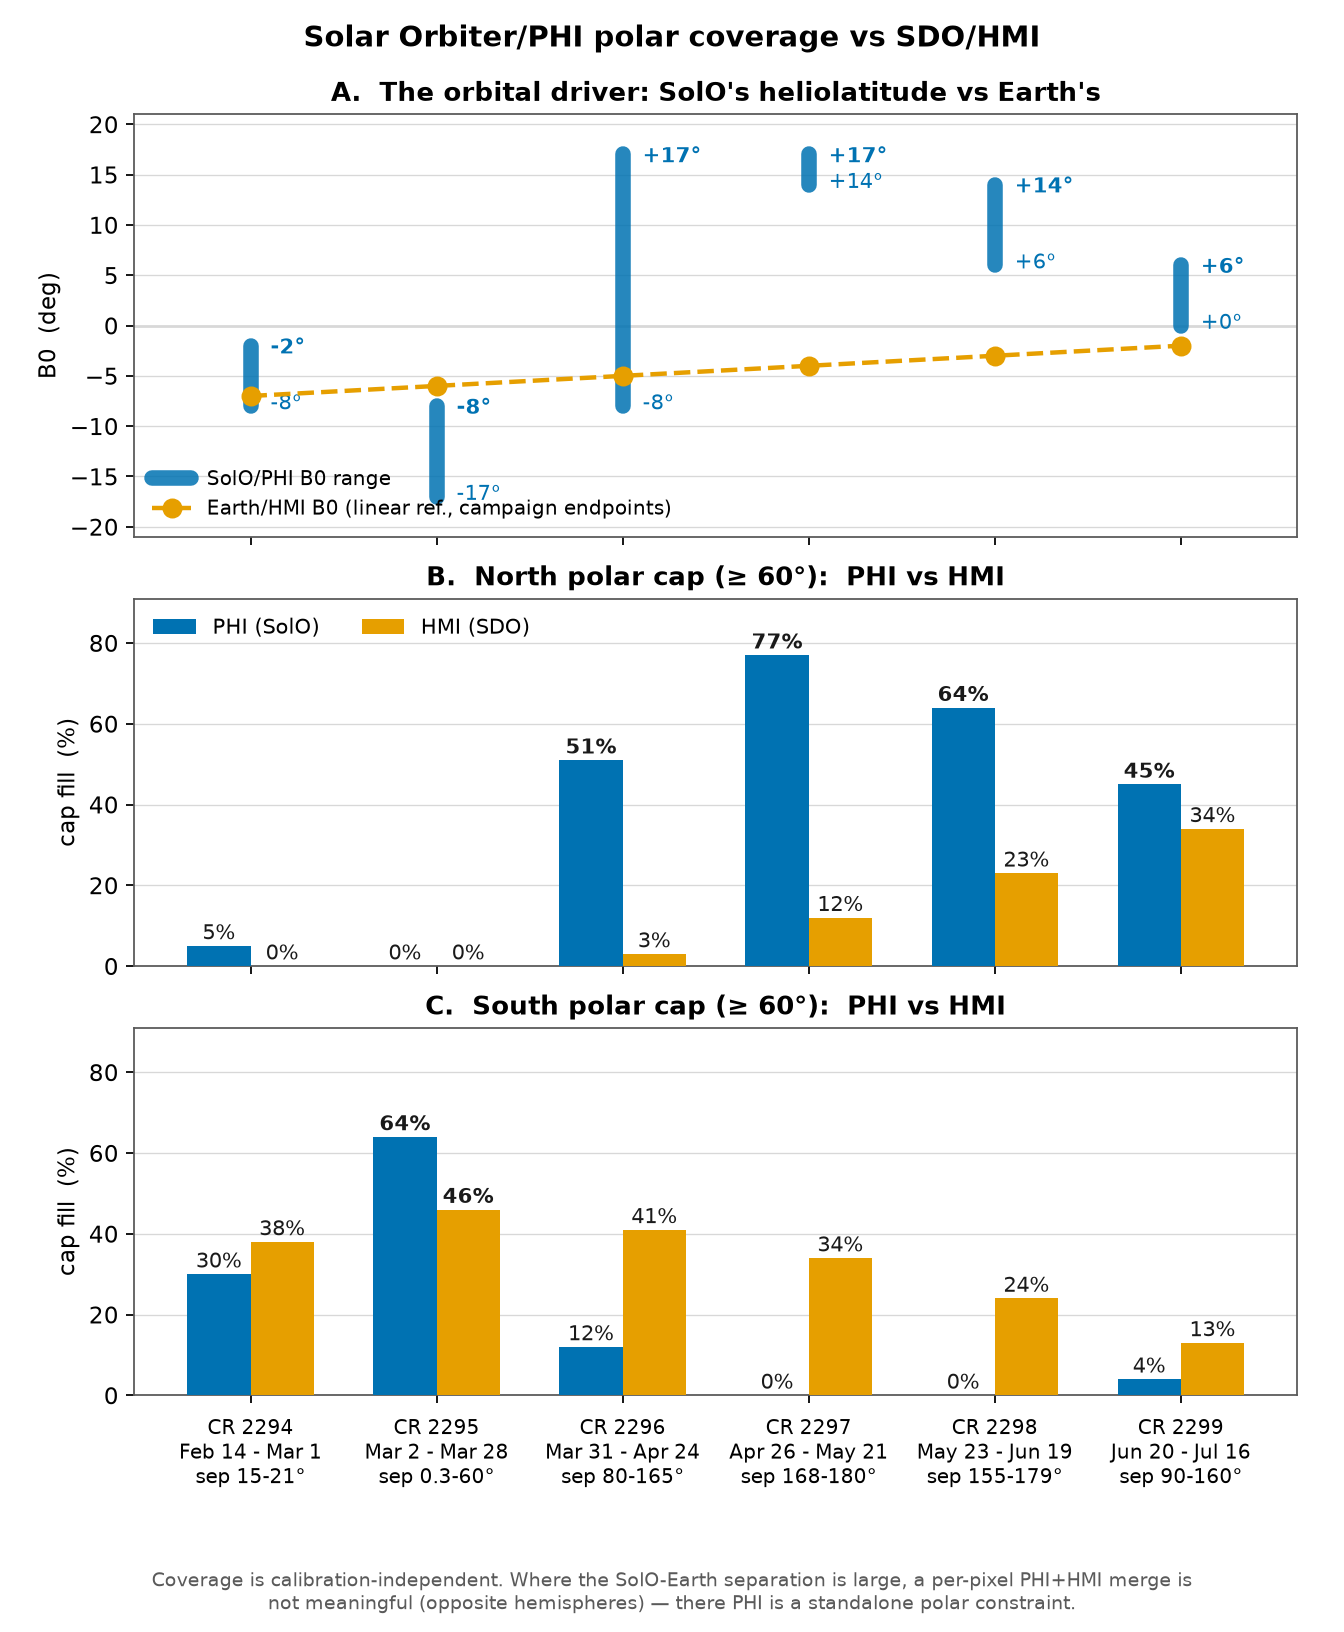
\includegraphics[width=\columnwidth]{figures/campaign_polar_advantage.png}
\caption{Solar Orbiter's $B_0$ excursion and the PHI-versus-HMI north/south polar-cap fill per rotation across the 2025 campaign, with the Solar Orbiter--Earth separation range annotated (Table~\ref{tab:campaign}). Earth's $B_0$ is shown as a linear reference between the campaign's stated endpoints, not a per-rotation measurement. Generated by \texttt{scripts/make\_campaign\_figure.py} directly from Table~\ref{tab:campaign}; \texttt{scripts/plot\_campaign\_summary.py} reproduces the same figure from a live \texttt{cr\_<N>/milestone/} pipeline run.}
\label{fig:campaign}
\end{figure}

The table uses the conservative limb cut $\mu_{\rm min} = 0.4$ (pixels within $\approx 66^{\circ}$ of disk centre only). The \emph{sign} of the advantage is robust, but its \emph{magnitude} depends on how much near-limb extrapolation is admitted: at $\mu_{\rm min} = 0.25$ (out to $\approx 76^{\circ}$), where the $1/\mu^{\alpha}$ conversion amplifies grazing-angle pixels unreliably, HMI's April north-cap fill rises from 3\% to 33\% and PHI's from 51\% to 86\%, so the ratio falls from $\approx 16\times$ to $\approx 2.6\times$ while PHI still leads. The order-of-magnitude figure is thus a statement about \emph{reliable} (high-$\mu$) coverage: under the cut where HMI's radial field is trustworthy it cannot constrain the cap at all, whereas PHI sees it near disk centre.

\subsection{Vantage effect on the dipole}
\label{sec:results-sign}

Where the two vantages share polar bins (CR\,2295 common support) they disagree on the \emph{sign} of the south-polar $g_{10}$ contribution (project mode: $+0.21$\,G for PHI versus $-0.10$\,G for HMI, on identical bins). A positive rescaling cannot flip a sign, so this is a genuine viewing-geometry effect: HMI's south-cap $B_r$ there is a near-limb $1/\mu^{\alpha}$ extrapolation, unreliable near solar maximum where the polar field is weak and reversing, whereas PHI sees the same bins close to disk centre and yields the better-constrained term.

The full CR\,2297 rotation sharpens this into a polarity statement. With PHI mapping 77\% of the north cap and HMI only 12\% (grazing-angle), PHI's north-cap dipole contribution is $g_{10,\rm north} = -0.25$\,G, matching the sign of the polar-filled reference chart for that rotation (total $g_{10} = -0.39$\,G; Sect.~\ref{sec:results-reference}) and of the expected cycle-25 north-pole reversal, whereas HMI's near-blind extrapolation gives $+0.19$\,G -- the opposite sign. Here the two vantages do not share the polar bins (the merged product is empty at $180^{\circ}$ separation), so this is not a common-support comparison but a direct measurement versus an extrapolation: that the polar-view measurement recovers the same polarity as the independent, community-standard chart, and the Earth-view extrapolation does not, is the coverage advantage expressed as a corrected polar-field sign.

\subsection{SFT impact: the payoff is where Earth is blind}
\label{sec:results-sft}

Because a per-pixel merge is invalid at the high-$B_0$ epochs, we inject PHI as a polar boundary constraint (Sect.~\ref{sec:methods-sft}): the SFT initial condition is HMI everywhere except the cap PHI observes, where PHI's zonal field is spliced in. Running with a cycle source ($\tau = 10$\,yr, 22\,yr integration, flux-balanced) on the pole PHI covers each rotation gives the results in Table~\ref{tab:sft}.

\begin{table}
\caption{SFT polar-constraint experiment results.}
\label{tab:sft}
\centering
\footnotesize
\begin{tabular}{lccc}
\hline\hline
Constraint & HMI fill & PHI field & $\Delta t_{\rm rev}$ \\
\hline
North (CR\,2296) & 3\%  & $-1.51$\,G\tablefootmark{a} & $-1.68$\,yr \\
North (CR\,2297) & 12\% & $-1.57$\,G\tablefootmark{a} & $-1.27$\,yr \\
South (CR\,2295) & 46\% & $0.20$ vs.\ $0.37$\,G\tablefootmark{b} & $-0.004$\,yr \\
\hline
\end{tabular}
\tablefoot{
\tablefoottext{a}{Injected PHI cap field; the co-temporal HMI cap field is $\approx 0$.}
\tablefoottext{b}{PHI cap field versus the co-observed HMI cap field.}
}
\end{table}

The two northern rotations both pull the first predicted reversal 1.3--1.7\,yr earlier ($\tau = 10$\,yr); the shift is robust to the assumed decay time (from $-1.68$ to $-1.50$\,yr for CR\,2296 between $\tau = 10$ and $\tau = 8$\,yr). The co-observed south cap does essentially nothing. Constraining the north cap, where HMI is effectively blind, injects a strong polar field where the Earth view has almost none, flips the initial dipole sign ($g_{10}(0) = -0.26$\,G versus $+0.10$\,G for HMI-only, CR\,2296), and pulls the first predicted polar reversal earlier across both northern rotations. It is the \emph{constrained} product, not PHI-only, that reverses earliest: PHI's north cap is strongly negative, so splicing it into an otherwise-HMI initial condition starts the dipole already below zero, on the verge of reversal, whereas the PHI-only and HMI-only profiles both start slightly positive and reverse about a year apart. In all cases the 22-yr dipoles converge to $\approx +3.1$\,G as the deterministic source dominates: the memory of the polar constraint lives in the reversal \emph{timing}, not the asymptote.

\begin{figure}
\centering
% 
\includegraphics[width=\columnwidth]{baseline_outputs/cr_2296/milestone/sft_polar/sft_polar_figure.png}
\fbox{\begin{minipage}[c][0.30\columnwidth][c]{0.92\columnwidth}
\centering\itshape\small
Figure not yet generated --- run \texttt{scripts/run\_sft\_polar\_experiment.py} and \texttt{scripts/plot\_sft\_polar.py}, then uncomment the \texttt{\textbackslash includegraphics} line above.
\end{minipage}}
\caption{HMI-only initial condition (flat near zero through the constrained cap) versus the HMI+PHI polar-constrained initial condition, and the resulting $g_{10}(t)$ with the $-1.68$\,yr reversal-timing shift. Reproduced by \texttt{scripts/run\_sft\_polar\_experiment.py} and \texttt{scripts/plot\_sft\_polar.py}; regenerate the pipeline outputs before compiling to populate this panel.}
\label{fig:sft}
\end{figure}

\subsection{Reference validation and its limit}
\label{sec:results-reference}

Checked per rotation against \texttt{hmi.synoptic\_mr\_polfil\_720s} \citep{Sun2018}, the standard chart's dipole holds near $-0.17$ to $-0.21$\,G through CR\,2294--2296, then declines sharply to $-0.57$\,G by CR\,2298 before a slight rebound to $-0.52$\,G at CR\,2299 (Table~\ref{tab:reference}), tracking the cycle-25 axial dipole rebuilding (negative) after the polar reversal. Early in the window, where the true dipole is near zero, the partial-coverage products do not reproduce its sign (all positive, $+0.3$ to $+1.0$\,G in project mode), because a near-zero dipole sampled from partial per-rotation longitude coverage is swamped by sampling noise, so the early-2025 \emph{absolute} $g_{10}$ magnitudes are provisional. As the true dipole strengthens, however, the products lock onto it: by CR\,2299 both PHI ($-0.19$\,G) and HMI ($-0.03$\,G) are negative, matching the reference sign, and PHI is now closer to the reference than HMI ($\Delta = +0.33$ versus $+0.49$\,G) -- the opposite of the early ordering. Once the north polar field is strong and negative, the vantage that actually sees it (PHI) recovers more of it than the Earth-view extrapolation, corroborating the CR\,2297 polarity result (Sect.~\ref{sec:results-sign}) from a second, independent direction.

\begin{table}
\caption{Axial dipole moment against the reference chart, project-fill mode.}
\label{tab:reference}
\centering
\footnotesize
\begin{tabular}{lccccc}
\hline\hline
Rotation & $g_{10,\rm ref}$ & $g_{10,\rm PHI}$ & $\Delta_{\rm PHI}$ & $g_{10,\rm HMI}$ & $\Delta_{\rm HMI}$ \\
\hline
CR\,2294 & $-0.21$ & $+0.47$ & $+0.68$ & $+0.35$ & $+0.57$ \\
CR\,2295 & $-0.17$ & $+0.98$ & $+1.15$ & $+0.34$ & $+0.50$ \\
CR\,2296 & $-0.18$ & $+0.56$ & $+0.74$ & $+0.17$ & $+0.36$ \\
CR\,2297 & $-0.39$ & $+0.29$ & $+0.68$ & $+0.12$ & $+0.50$ \\
CR\,2298 & $-0.57$ & $+0.11$ & $+0.67$ & $-0.01$ & $+0.55$ \\
CR\,2299 & $-0.52$ & $-0.19$ & $+0.33$ & $-0.03$ & $+0.49$ \\
\hline
\end{tabular}
\tablefoot{All values in G. $g_{10,\rm ref}$ is from \texttt{hmi.synoptic\_mr\_polfil\_720s}; $\Delta_X = g_{10,X} - g_{10,\rm ref}$. From \texttt{scripts/compare\_reference\_by\_rotation.py} (\texttt{data/reference\_dipole\_by\_rotation.csv}). The merged product has valid rows only for CR\,2294--2295 (Sect.~\ref{sec:methods-guard}); for CR\,2296--2299 the Solar Orbiter--Earth separation exceeds the merge guard and no merged product exists.}
\end{table}

%-------------------------------------------------------------------
\section{Discussion}
\label{sec:discussion}

The organising result of the campaign is a correlation not initially anticipated: PHI's polar advantage is largest exactly when the Solar Orbiter--Earth separation is largest, because both are driven by the same orbital motion -- Solar Orbiter reaches high heliolatitude precisely when it is far around the Sun from Earth. This has a sharp methodological consequence. When the separation is small (February, and the mid-March near-conjunction) a per-pixel PHI+HMI merge is well posed, but PHI then carries little polar advantage; when PHI's advantage is decisive (the April--May north cap) the separation is $80^{\circ}$--$172^{\circ}$ and a merge is meaningless.

The two vantages are therefore complementary in \emph{time}, not co-registered in \emph{space}. The scientific value of the polar view is not as a pixel-level merge partner for HMI, but as an independent polar constraint -- a boundary condition for the SFT model -- at the epochs Earth cannot see a given pole. The $-1.68$\,yr reversal shift from the north-cap constraint, set against the null result from the co-observed south cap, is the concrete expression of this: the added vantage matters only, but decidedly, where the Earth view is blind. The separation guard (Sect.~\ref{sec:methods-guard}) is what makes the statement rigorous, by refusing to construct a blended product from two disjoint hemispheres.

%-------------------------------------------------------------------
\section{Uncertainties and limitations}
\label{sec:uncertainties}

\begin{itemize}
    \item \emph{Line-of-sight-to-radial approximation.} $B_r \approx B_{\rm los}/\mu^{\alpha}$ is poor on strong active-region fields; a quiet-Sun restriction ($|B_r| \le 50$\,G) shrinks the cross-vantage project-mode gap, and vector inversions would remove this error class. The $\alpha$ sensitivity is sub-dominant: over $\alpha = 0.6$--1.0 the PHI dipole varies by only $\approx 3\%$ (0.31 to 0.30\,G) and the HMI dipole by $\approx 9\%$ (0.37 to 0.40\,G), smaller than the case-to-case scatter and far smaller than the fill-mode spread below.
    \item \emph{Calibration slope is a resolution effect.} The sub-unity PHI-versus-HMI slope ($\approx 0.56$, declining with Solar Orbiter--Sun distance) is closed by degrading HMI to PHI's resolution: the slope rises to unity near 5\,px FWHM while the correlation peaks at 2--3\,px (Sect.~\ref{sec:data-systematics}). It is a plate-scale effect, not an instrument-scale or vantage error.
    \item \emph{Coverage cut.} The polar-advantage \emph{magnitude} depends on the limb cut $\mu_{\rm min}$ (Sect.~\ref{sec:results-coverage}): $\approx 16\times$ at the conservative $\mu_{\rm min} = 0.4$ versus $\approx 2.6\times$ at $\mu_{\rm min} = 0.25$, where HMI admits grazing-angle polar pixels of low reliability. The sign of the advantage is robust to the cut.
    \item \emph{Longitude coverage.} Per-rotation windows have partial longitude coverage, which dominates the uncertainty on the \emph{absolute} 2025 $g_{10}$ (Sect.~\ref{sec:results-reference}); denser PHI synoptic programmes would close this. Differential and coverage statements are robust against it.
    \item \emph{Fill-mode dependence} remains the largest single uncertainty on absolute $g_{10}$; product-versus-product statements are robust against it.
    \item \emph{One-dimensional (axisymmetric) SFT.} Longitude-dependent assimilation, and time-dependent assimilation of PHI beyond a single initial condition, are left to future work.
\end{itemize}

%-------------------------------------------------------------------
\section{Conclusions}
\label{sec:conclusions}

\begin{enumerate}
    \item Merged PHI+HMI synoptic maps are constructible and validated at small Solar Orbiter--Earth separation (map-space $r \approx 0.9$ between independent vantages; $\approx 0.05$\,G common-support dipole agreement).
    \item In the 2025 high-$B_0$ campaign, PHI's polar-cap coverage overtakes HMI by up to $16\times$ (north cap 51\% versus 3\% in April), and the advantage switches on with Solar Orbiter's heliolatitude exactly as hypothesised -- south cap in March, north cap in April -- strengthening to 77\% versus 12\% across the full CR\,2297 rotation at the northern apex, then switching off symmetrically as Solar Orbiter descends and Earth's $B_0$ rises: the advantage is governed by the difference of the two heliolatitudes. With apex coverage, PHI recovers the negative sign of the reversing cycle-25 north polar field, matching the community-standard chart, which the Earth-view extrapolation gets wrong; by CR\,2299 PHI's total dipole is also closer to the reference chart than HMI's.
    \item PHI's polar advantage is largest where the Solar Orbiter--Earth separation is largest, so at the decisive epochs the value of the polar view is as a standalone polar constraint, not a co-registered merge partner. The two vantages are complementary in time, not in space.
    \item Adding PHI's north-cap constraint at the epoch where HMI is blind (3\% fill) shifts the first SFT-predicted polar reversal by $-1.68$\,yr; adding its south-cap constraint where HMI co-observes (46\% fill) changes nothing ($-0.004$\,yr). The polar view moves the prediction only where the Earth view lacks the information.
    \item The methodology, its systematics (orientation, calibration, deprojection, polar filling, co-observation separation), and the open-source tooling are established end to end, from data download through the polar-constrained SFT experiment.
\end{enumerate}

%-------------------------------------------------------------------
\begin{acknowledgements}
The author thanks the Solar Orbiter/PHI and SDO/HMI instrument teams for the public availability of the data used in this work.
\end{acknowledgements}

\paragraph{Data availability.}
The SO/PHI-FDT magnetograms are publicly available from the ESA Solar Orbiter Archive (SOAR, \url{soar.esac.esa.int}); the SDO/HMI magnetograms are publicly available from the Joint Science Operations Center (JSOC, \url{jsoc.stanford.edu}). The open-source analysis pipeline, baseline configuration, and scripts used to reproduce every result reported here are available in the project repository.

\bibliographystyle{aa}
\bibliography{references}

\end{document}
